\chapter{Semiconductor model}

In this chapter we present the basic physical properties of semiconductor material accordingly with the quantum mechanics theory \citep{ModernVLSIdevices} and the Drift-Diffusion model.

\section{Basic Device Physics}

As the most used material in the fabrication of VLSI devices is silicon, the description of physics is based on this material choice.

\subsection{Intrinsic semiconductor}
In a silicon crystal each atom has four valence electrons to share with its four nearest neighboring atoms. The valence electrons are shared in a paired configuration called covalent bond.  The description of electrons in a solid, made by the quantum mechanics, is that the allowed energy levels of electrons are grouped into bands separated by regions of not allowed energy: forbidden gaps. The highest energy band completely filled by electron at 0[K] is called the \textit{valence band} ($E_V$), the next energy band levels are called \textit{conduction band} ($E_C$).

\begin{figure}[!h]
\centering
\subfloat[][Metal]
{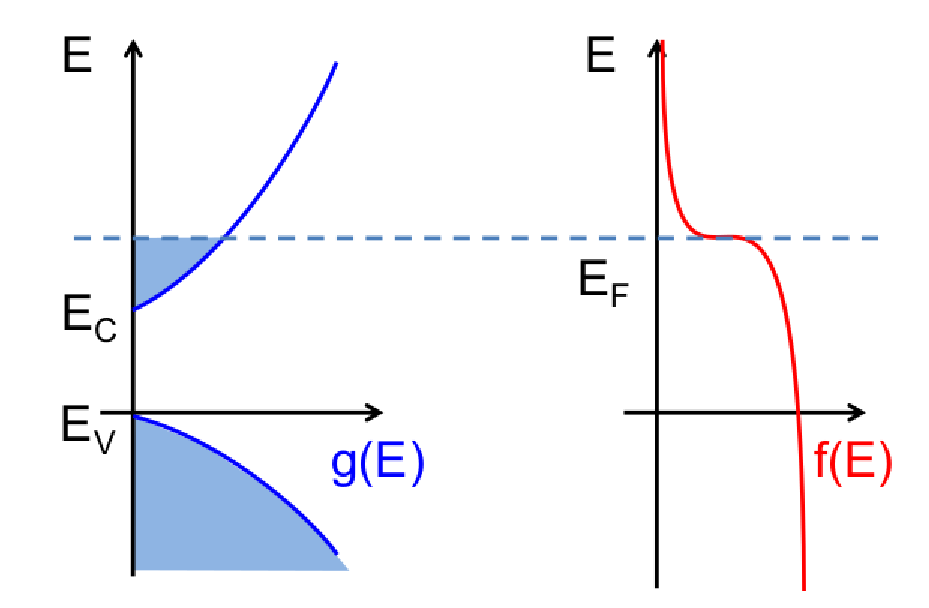
\includegraphics[width=.45\textwidth]{SemiconductorModel/BandeMetalli.eps}}
\psp{5}
\subfloat[][Insulator]
{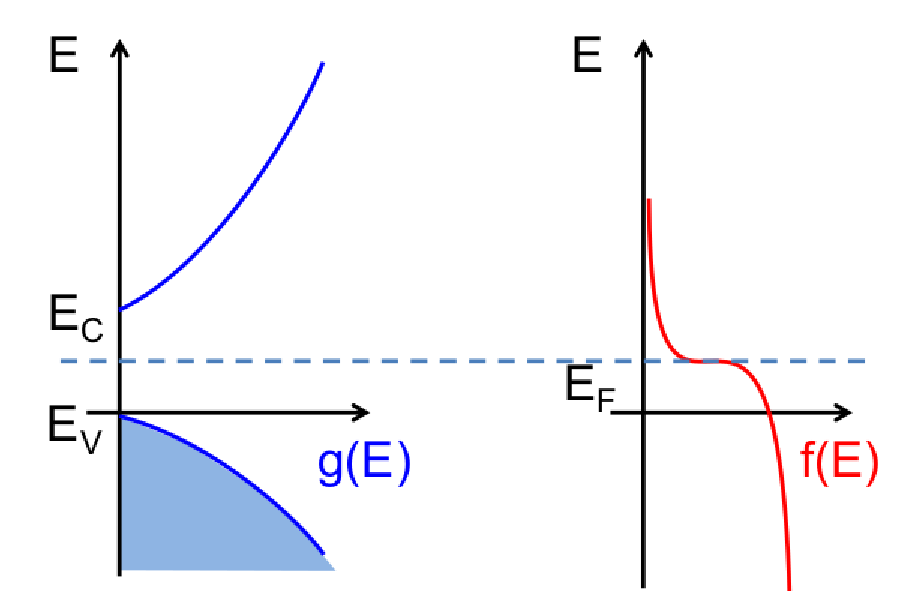
\includegraphics[width=.45\textwidth]{SemiconductorModel/BandeSemiconduttori.eps}}
\caption{Two typical examples of state density occupation (g(E)) and probability distribution (f(E)).  }
\end{figure}

Because in silicon the band gap is 1.11 [eV] \cite{SolidState} also at room temperature a small fraction of the electrons are excited into the conduction band, leaving behind vacancies (called \textit{holes}) in the valence band.
In contrast, an insulator has a much larger forbidden gap making room-temperature conduction virtually impossible, while metals have partially filled conduction bands even at absolute zero temperature, this make them good conductors at any temperature. 

A suitable formulation of the electron concentration is given (for holes is symmetric) by the follow integral:
\begin{equation}
\label{eq: carrier densiy integral}
n = \int_{E_c}^\infty g(E)f(E) \, dE
\end{equation}
With $g(E)dE$ we indicate the number of electronic states per unit volume with an energy between $E$ and $E+dE$ in the conduction band and $f(E)$ is the \textit{Fermi-Dirac distribution function}, which gives the probability that an electronic state at energy E is occupied by an electron,
\begin{equation}
\label{eq: fermi dirac distribution}
f_D(E) = \dfrac{1}{1+exp\left(\dfrac{E-E_f}{k_BT}\right)} 
\end{equation}
here $k_B=1.38\times10^{-23}[J/K]$ is Boltzmann's constant, $T$ is the absolute temperature and $E_f$ is the \textit{Fermi level}. In general \referenzaeq{eq: carrier densiy integral} is a Fermi integral of the order $1/2$ and must be evaluated numerically.
 
\begin{Definizione}
The Fermi level ($E_f$) is the energy at which the probability of occupation of an energy state by an electron is exactly one-half.
\end{Definizione}

In most cases when the energy is at least several $k_BT$ above or below the Fermi level (case of non degenerate semiconductor), equation \referenzaeq{eq: fermi dirac distribution} can be approximated by the Maxwell-Boltzmann statistics for classical particles, which reads as follows:

\begin{equation}
\label{eq: maxwell distribution}
f_D(E)\simeq f_{MB}(E) = 
\begin{cases}
exp\left(-\dfrac{E-E_f}{KT}\right) & E\gg E_f \\
1-exp\left(-\dfrac{E_f-E}{KT}\right) & E \ll E_f
\end{cases}
\end{equation}

Fermi level plays an essential role in characterizing the equilibrium state of a stystem, it is important to keep in mind the follow observation.

\begin{Osservazione}
When two systems are in thermal equilibrium with no current flow between them, their Fermi levels must be equal: in other words for a continuous region (of metals or semiconductors in contact), the Fermi level at thermal equilibrium is flat (spatially constant throughout the region).
\end{Osservazione}

Considering \referenzaeq{eq: carrier densiy integral} with \referenzaeq{eq: maxwell distribution} the analytical results of the integration is

\begin{align}
n & = N_c exp\left(-\dfrac{E_c-E_f}{KT}\right) \label{eq: n density fd}\\
p & = N_v exp\left(-\dfrac{E_f-E_v}{KT}\right)  \label{eq: p density fd}
\end{align}

where $N_c$ and $N_v$ are the \textit{effective density of states}.
In intrisic semiconductor $n=p$ and the \textit{intrinsic Fermi level} $E_i$ can be calculated using equations \referenzaeq{eq: n density fd} and \referenzaeq{eq: p density fd} as:

\begin{equation}
\label{eq: midgap equilibrium}
E_i=E_f=\dfrac{E_c+E_v}{2} - \dfrac{KT}{2}ln\left(\dfrac{N_c}{N_v}\right)
\end{equation}

By replacing \referenzaeq{eq: midgap equilibrium} in \referenzaeq{eq: n density fd} we have the expression of the intrinsic carrier concentration $n_i=n=p$:


\begin{equation}
\label{eq: ni equilibrium NcNv}
n_i = \sqrt{N_cN_v}exp\left(-\dfrac{E_g}{2KT}\right)
\end{equation}

\begin{Osservazione}
Since the thermal energy, $k_BT$ is much smaller than the usual semiconductor bandgap $E_g$, the intrinsic Fermi level is very close to the midpoint between the conduction band and the valence band.
\end{Osservazione}

Equations \referenzaeq{eq: n density fd} and \referenzaeq{eq: p density fd} can be rewritten in terms of the intrinsic carrier density ($n_i$) and energy ($E_i$) :

\begin{align}
n & = n_i exp\left(\dfrac{E_f-E_i}{KT}\right) \label{eq: n density mb}\\
p & = n_i exp\left(\dfrac{E_i-E_f}{KT}\right)  \label{eq: p density mb}
\end{align}

Finally we remark a fundamental and useful relation holds at the thermical equilibrium

\begin{equation}
\label{eq: legge di azione di massa}
np=n_i^2
\end{equation}

this relation is usually note as \textit{mass action law}.

The analysis of the work principles of devices can be effective done by the band diagram (\figref{fig: band diagram}), which summarizes the informations presented above.
\begin{figure}[!h]
\centering
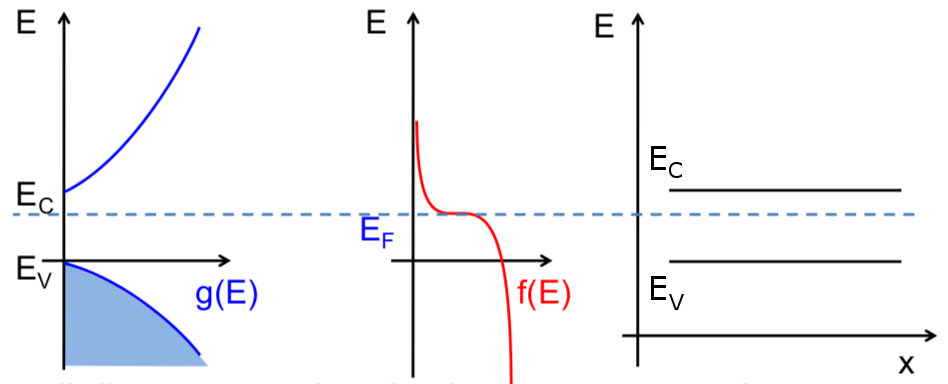
\includegraphics[width=.8\textwidth]{SemiconductorModel/DiagrammaBande.png}
\caption{Construction of tha band diagram.}
\label{fig: band diagram}
\end{figure}

\subsection{Extrinsic semiconductor}
At room temperature intrinsic semiconductor has an extremely low free-carrier concentration, therefore, its resistivity is very high. In order to make semiconductor a better conductor impurities atoms are added which introduce additional energy levels in the forbidden gap: these impurities are easily ionized adding either electrons to the conduction band or holes to the valence band. Here the electrical conductivity is dominated by the type and concentration of the impurity atoms.

In the case of silicon two are the types of impurities which are electrically active: those from column V such as arsenic or phosphorus, and those from column III such as boron or indium.

 In most cases, the thermal energy at room temperature is sufficient to ionize the impurities and free the extra electron to the conduction band (column V) or accepting an electron from valence band (column III). Column V impurities are called \textit{donors}; they become positively charged when ionized. Silicon material doped with column-V impurities or donors is called \textit{n-type} silicon.

Column III impurities are called \textit{acceptors}: they become negatively charged when ionized. Silicon material doped with column-III impurities or acceptors is called \textit{p-type} silicon.

A p-type or an n-type is named as \textit{extrinsic} silicon.
In terms of the energy-band diagrams, donors add allowed electron states in the bandgap close to the conduction-band edge, while acceptors add allowed states just above the valence-band edge.

The Fermi level in n-type silicon moves up towards the conduction band while in p-type silicon moves down towards the valence band.
The exact position of the Fermi level depends on both the ionization energy and the concentration of dopants. For the sake of simplicity we consider that at room temperature all impurties are ionized ($N_d = N_d^+$ and $N_a = N_a^-$).  For an n-type material with a donor impurity concentration, $N_d$, the charge neutrality condition requires that
\begin{equation}
\label{eq: equilibrium charge in n-type}
n = N_d^+ + p
\end{equation}
 where $N_d^+$ is the density of ionized donors.  Similarly for a p-type material with acceptor impurity concentration $N_a$ we have
\begin{equation}
\label{eq: equilibrium charge in p-type}
p = N_a^- + n
\end{equation}
 
 Because the magnitude of impurities is between $10^{16}\div 10^{20} [cm^{-3}]$, and intrinsic carrier concentration in the order of $10^{10}[cm^{-3}]$, in typical case we can approximate the \referenzaeq{eq: legge di azione di massa} as:
  
\begin{equation}
\label{eq: equilibiurm approximation}
\begin{array}{ll}
n \simeq N_d & p \simeq \dfrac{n_i^2}{N_d} \\ \\
p \simeq N_a & n \simeq \dfrac{n_i^2}{N_a}
\end{array}
\end{equation}

Replacing \referenzaeq{eq: equilibiurm approximation} in  \referenzaeq{eq: n density fd} and \referenzaeq{eq: p density fd} in \referenzaeq{eq: equilibrium charge in n-type} and \referenzaeq{eq: equilibrium charge in p-type} and solving the algebraic equation we have
 
 \begin{align}
 E_c-E_f = KTln\left(\dfrac{N_c}{N_d}\right)  \label{eq: Ef in n-type}\\
 E_f-E_v= KTln\left(\dfrac{N_v}{N_a}\right) \label{eq: Ef in p-type}
 \end{align}

Equation \referenzaeq{eq: Ef in n-type} and \referenzaeq{eq: Ef in p-type} can be written in a more useful form using \referenzaeq{eq: ni equilibrium NcNv} and \referenzaeq{eq: midgap equilibrium} (for $n_i$ and $E_i$):

 \begin{align}
 E_f-E_i = KTln\left(\dfrac{N_d}{n_i}\right)  \label{eq: Ef in n-type Ei} \\
 E_i-E_f = KTln\left(\dfrac{N_a}{n_i}\right)  \label{eq: Ef in p-type Ei} 
 \end{align}

\begin{Osservazione}
The distance between the Fermi level and the intrinsic Fermi level (near the midgap) is a logarithmic function of doping concentration.
\end{Osservazione}


\begin{figure}[!h]
\centering
\subfloat[][n-type]
{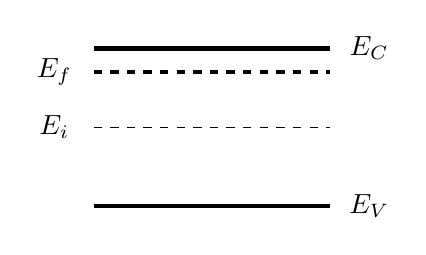
\begin{tikzpicture}
[scale=1.0]
\def\Ecxa{0.0}
\def\Ecya{2}
\def\Ecxb{3}
\def\Ecyb{2}

\def\Evxa{\Ecxa}
\def\Evya{0}
\def\Evxb{\Ecxb}
\def\Evyb{0}

\def\Efxa{\Ecxa}
\def\Efya{1.7}
\def\Efxb{\Ecxb}
\def\Efyb{1.7}

\def\Eixa{\Ecxa}
\def\Eiya{1}
\def\Eixb{\Ecxb}
\def\Eiyb{1}

\node at (\Ecxb+0.5,\Ecyb){$E_C$};
\node at (\Evxb+0.5,\Evyb){$E_V$};
\node at (\Efxa-0.5,\Efya){$E_f$};
\node at (\Eixa-0.5,\Eiya){$E_i$};

\draw[ultra thick](\Ecxa,\Ecya)--(\Ecxb,\Ecyb);
\draw[ultra thick](\Evxa,\Evya)--(\Evxb,\Evyb);
\draw[ultra thick,dashed](\Efxa,\Efya)--(\Efxb,\Efyb);
\draw[dashed](\Eixa,\Eiya)--(\Eixb,\Eiyb);
\end{tikzpicture}}
\psp{20}
\subfloat[][p-type]
{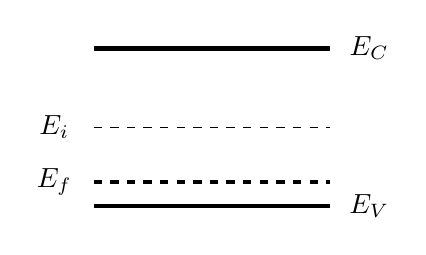
\begin{tikzpicture}
[scale=1.0]
\def\Ecxa{0.0}
\def\Ecya{2}
\def\Ecxb{3}
\def\Ecyb{2}

\def\Evxa{\Ecxa}
\def\Evya{0}
\def\Evxb{\Ecxb}
\def\Evyb{0}

\def\Efxa{\Ecxa}
\def\Efya{0.3}
\def\Efxb{\Ecxb}
\def\Efyb{0.3}

\def\Eixa{\Ecxa}
\def\Eiya{1}
\def\Eixb{\Ecxb}
\def\Eiyb{1}

\node at (\Ecxb+0.5,\Ecyb){$E_C$};
\node at (\Evxb+0.5,\Evyb){$E_V$};
\node at (\Efxa-0.5,\Efya){$E_f$};
\node at (\Eixa-0.5,\Eiya){$E_i$};

\draw[ultra thick](\Ecxa,\Ecya)--(\Ecxb,\Ecyb);
\draw[ultra thick](\Evxa,\Evya)--(\Evxb,\Evyb);
\draw[ultra thick,dashed](\Efxa,\Efya)--(\Efxb,\Efyb);
\draw[dashed](\Eixa,\Eiya)--(\Eixb,\Eiyb);
\end{tikzpicture}}
\caption{Band diagrams of estrinsic silicon for \referenzaeq{eq: Ef in n-type Ei} and \referenzaeq{eq: Ef in p-type Ei}.}
\label{fig: Band diagrams of estrinsic silicon}
\end{figure}

\subsection{Densities at nonequilibrium condition}

In VLSI device a nonequilibrium condition is often possible where the densities of one or both types of carriers depart from their equilibrium values given by \referenzaeq{eq: n density mb} and \referenzaeq{eq: p density mb}.
In particular, the minority carrier concentration can be easily overwhelmed by injection from neighboring regions. Under these circumstances, while the electrons and holes are in local equilibrium with themselves, they are not in equilibrium with each other. In order to extend the relationship between Fermi level and densities discussed above, we can introduce different Fermi levels for electrons and holes. They are called \textit{quasi Fermi levels} defined as follow

\begin{align}
E_{fn} = E_i + k_B T ln\left( \dfrac{n}{n_i} \right) \label{eq: quasi fermi level electron} \\
E_{fp} = E_i - k_B T ln\left( \dfrac{p}{n_i} \right) \label{eq: quasi fermi level hole}
\end{align}


Considering the well known relation between electrostatic potential and energy \referenzaeq{eq: quasi fermi level electron} and \referenzaeq{eq: quasi fermi level hole} can be written as

\begin{align}
n & = n_i exp\left(\dfrac{\varphi_{i}-\varphi_n}{k_BT/q}\right) \label{eq: non eq n density mb}\\
p & = n_i exp\left(\dfrac{\varphi_p-\varphi_{i}}{k_BT/q}\right)  \label{eq: non eq p density mb}
\end{align}

where $\varphi_n$ and $\varphi_p$ are the quasi fermi electrostatic potential levels and $\varphi_i$ is the midgap electrostatic potential level. 

\begin{Osservazione}
In non equilibrium condition quasi Fermi levels have the same physical interpretation in terms of the state occupancy as the Fermi level, therefore the electron (hole) density in the conduction band can be calculated using $E_{fn}$ ($E_{fp}$).
\end{Osservazione}

\subsection{Carrier transport in semiconductor}
\label{sec: carrier transport}

Carrier transport or current flow in silicon is driven by two different mechanisms:
\begin{itemize}
\item the \textbf{drift} of carriers, which is caused by the presence of an electric field;
\item the \textbf{diffusion} of carriers, which is caused by and electron or hole concentration gradient.
\end{itemize}

\subsubsection{Drif current - Ohm's law}

When an electric field is applied to a silicon device, the free carriers are accelerated and acquire a drift velocity superimposed upon their random thermal motion.

\begin{Osservazione}
The drift velocity of holes ($h$) is in the direction of the applied field, and the drift velocity of electrons ($e$) is opposite to the field.
\end{Osservazione}

The velocity of the carriers does not increase indefinitely under field acceleration, since they are scattered frequently and lose their acquired momentum after each collision.
During their motion throughout the lattice structure, carriers travel at an average speed definded by
\begin{equation}
\label{eq: velocities}
\vect{v}_d^e = - \dfrac{q\vect{E}\tau_e}{m_e}  \psp{20} 
\vect{v}_d^h = + \dfrac{q\vect{E}\tau_h}{m_h}
\end{equation}

where $q=1.602e^{-19}[C]$ is the elementary charge, $\vect{E}$ the electric field, $\tau_e$, $\tau_h$ the average time between two consecutive scattering events and $m_e$, $m_h$ are the effective mass.
The coefficient $q\tau_e / m_e$ ($q\tau_p / m_p$) characterizes how quickly a carrier can move through the lattice and it's well known as carrier mobility $[m^2V^{-1}s^{-1}]$.
In general, to include different scattering mechanism to the mobility the \textit{Matthiessen's rule} is used:
\begin{equation}
\dfrac{1}{\mu} = \dfrac{1}{\mu_L} + \dfrac{1}{\mu_I} + \cdots
\end{equation}
where $\mu_L$ and $\mu_I$ correspond to the lattice and impurity scattering (for a more detailed description of mobility models see \cite{ModernVLSIdevices}). 

Therefore the drift electron (hole) current density, reads as follows:

\begin{align}
\vect{J}_n =& -qn\vect{v}_d^n = qn\mu_n\vect{E}   = \sigma_n\vect{E} \label{eq: drift electron} \\ 
\vect{J}_p =& +qp\vect{v}_d^p = qp\mu_p\vect{E} = \sigma_p\vect{E} \label{eq: drift hole}
\end{align}

The scalar coefficient $qn\mu_n(qp\mu_p)$ is called electron (hole) conductivity $\sigma_n(\sigma_p)$. 

Relations \referenzaeq{eq: drift electron} and \referenzaeq{eq: drift hole} expresses the well known \textit{Ohm' law} stating that the current density is directly proportional to the applied electric field.


\subsubsection{Diffusion current - Fick's law}

In semiconductor devices it's usual have different profiles of dopant in order to allow particular behaviors, this implies a not uniform concentration of carriers which they also diffuse as a result of the concentration gradient. This leads to an additional current contribution accordingly to the \textit{Fick's law}:
\begin{align}
\vect{J}_n = -D_n(-q\nabla n) \label{eq: diff electron}\\
\vect{J}_p = -D_p(+q\nabla p) \label{eq: diff hole}
\end{align}

The constants $D_n$ and $D_p$ are called electron and hole diffusion coefficients and have units of $[cm^2s^{-1}]$. Drift and diffusion are closely associated with the random thermal motion of carriers and their collisions with the silicon lattice in thermal equilibrium. The \textit{Einstein relation} \referenzaeq{eq: einstein relation} expresses the relation between diffusivity and mobility

\begin{equation}
\label{eq: einstein relation}
D_\eta = \dfrac{k_BT}{q}\mu_\eta.
\end{equation}

\subsubsection{Drift-Diffusion transport equations}
\label{subsub:driftdiffusion transport}

By considering \referenzaeq{eq: drift electron}, \referenzaeq{eq: drift hole}, \referenzaeq{eq: diff electron} and \referenzaeq{eq: diff hole}, the total electron and hole current densities become:

\begin{align}
\vect{J}_n &= qn\mu_n\vect{E} + qD_n\nabla n  \label{eq: drift diff electron}\\ 
\vect{J}_p &= qp\mu_p\vect{E} - qD_p \nabla p \label{eq: drift diff hole}
\end{align}
The total conduction current density is $\vect{J}=\vect{J}_n+\vect{J}_p$.

Equations \referenzaeq{eq: drift diff electron} and \referenzaeq{eq: drift diff hole} are called constitutive laws and they can be rewritten in two other ways highlighting different physical explanations of the same phenomenon. These reinterpreations give also different start points for the discrete solver algorithm.

Considering that electric field is related to the scalar potential as:
\begin{equation}
\label{eq: relazione pot electric}
\vect{E}  = -\nabla \varphi
\end{equation}

using \referenzaeq{eq: einstein relation} the current densities can be written as:

\begin{align}
\vect{J}_n &= -qn\mu_n\left(\nabla \varphi - \dfrac{k_BT}{qn}\nabla n \right) \label{eq: Jn DD} \\ 
\vect{J}_p &= -qp\mu_p\left(\nabla \varphi+ \dfrac{k_BT}{qp} \nabla p \right) \label{eq: Jp DD}
\end{align}

Considering equations \referenzaeq{eq: non eq n density mb} and \referenzaeq{eq: non eq p density mb} the above can be written as:

\begin{align}
\vect{J}_n = -qn\mu_n\nabla \varphi_n \label{eq: Jn qf}\\
\vect{J}_p = -qp\mu_p\nabla \varphi_p \label{eq: Jp qf}
\end{align}

With these equations we underlying an important aspect which occur in semiconductor material:
\begin{Osservazione}
The current density is proportional to the gradient of the quasi Fermi potential.
\end{Osservazione}

The third way to represent the current density is based on \textit{Slotboom variables} which are particularly suited for the semiconductor equations.

\begin{align}
u_n &= n_iexp\left(-\dfrac{\varphi_n}{V_{th}} \right) \label{eq: un slotboom} \\
u_p &= n_iexp\left(\dfrac{\varphi_p}{V_{th}} \right) \label{eq: up slotboom} 
\end{align}

where $V_{th}=k_BT/q$. Using the above equations into \referenzaeq{eq: drift diff electron} and \referenzaeq{eq: drift diff hole} we obtain:

\begin{align}
\vect{J}_n &= qD_n exp\left(\dfrac{\varphi}{V_{th}}\right) \nabla u_n \label{eq: Jn slotboom} \\
\vect{J}_p &= -qD_p exp\left(-\dfrac{\varphi}{V_{th}}\right)  \nabla u_p \label{eq: Jp slotboom}
\end{align}

\begin{Osservazione}
The drift-diffusion current density in a semiconductor, is a totally diffusive flux of a new kind of carrier with a proper diffusion coefficient. 
\end{Osservazione}


\section{Drift Diffusion Model for semiconductor}
\label{section: dd model for semi}

Simulations on integrated devices works on several different scale, the \textit{Drift Diffusion model} (DD) is the most widely used mathematical tool for industrial simulaiton of semiconductor devices. In this section we'll show how is possible to deduce the DD model.

\subsection{Drift Diffusion formulation}
 The system of Maxwell equations describes the propagation of electromagnetic signal in a medium:

\begin{align}
\nabla \times \vect{H} & =  \vect{J} + \dfrac{\partial \vect{D}}{\partial t} \label{eq: magnetic equation} \\ 
\nabla \times \vect{E} & =  - \dfrac{\partial \vect{B}}{\partial t} \label{eq: ampere law}\\ 
\nabla \cdot \vect{D} & =  \rho \label{eq: gauss law}\\ 
\nabla \cdot \vect{B} &  =  0 \label{eq: no magetic charge law}
\end{align}

with the following set of constitutive laws that characterize the electromagnetic properties of the medium:

\begin{equation}
\begin{array}{rcl}
\vect{D} & = & \epsilon \vect{E} \\
\vect{B} & = & \mu_m \vect{H} \label{eq: magnetic costitutive}
\end{array}
\end{equation}

where $\epsilon$ is the material dielectric permettivity $[F cm^{-1}]$ and $\mu_m$ is the magnetic permeability $[H cm^{-1}]$. Since $\nabla \cdot (\nabla \times \vect{A})=0$ for any vector $\vect{A}$, \referenzaeq{eq: no magetic charge law} is satisfied by introducing a vector potential $\vect{A}$ such that $\vect{B}= \nabla \cdot \vect{A}$. We replace it in \referenzaeq{eq: ampere law} obtains

\begin{equation}
\nabla \times \left( \vect{E} + \dfrac{\partial \vect{A}}{\partial t} \right) = 0.
\end{equation}

From this we can state that exist a scalar potential $\varphi$ such that

\begin{equation}
\label{eq: potenziale scalare}
\vect{E} + \dfrac{\partial \vect{A}}{\partial t} = -\nabla \varphi
\end{equation}


 Applying the divergence operator and we obtain using \referenzaeq{eq: relazione pot electric}, \referenzaeq{eq: magnetic costitutive} and \referenzaeq{eq: gauss law};  \referenzaeq{eq: potenziale scalare} becomes

\begin{equation}
\rho + \dfrac{\partial \vect{A}}{\partial t}  = -\nabla \cdot (\epsilon \nabla \varphi)
\end{equation}

We now assume that $\dfrac{\partial \vect{A}}{\partial t} = 0$ (quasi static approximation) and we have the \textit{Poisson Equation}

\begin{equation}
\label{eq: Poisson equation}
\nabla \cdot (\epsilon \nabla \varphi) = \rho.
\end{equation} 
	
Applying the divergence operator on the equation \referenzaeq{eq: magnetic equation}  and we get the \textit{Continuity Equation}

\begin{equation}
\label{eq: continuity equation total}
\dfrac{\partial \rho}{\partial t} + \nabla \cdot \vect{J}  =  0 \end{equation} 




To close the above system (\referenzaeq{eq: Poisson equation} and \referenzaeq{eq: continuity equation total} ), we need to specify the mathematical form of the electric charge density ($\rho$) and the electric conduction current density ($\vect{J}$).
Considering \referenzaeq{eq: equilibiurm approximation} $\rho$ can be expressed by \referenzaeq{eq: charge balance}


\begin{equation}
\label{eq: charge balance}
\rho = \underbrace{q(p-n)}_{\rho_{free}} +\underbrace{q(N_D-N_A)}_{\rho_{fixed}}
\end{equation}

\begin{itemize}
\item free charge ($\rho_{free}$) (free electron and holes carriers),
\item fixed charge ($\rho_{fixed}$) (ionoized dopant impurities).
\end{itemize} 


 Notice that we assume $N_D$ and $N_A$ time invariant ($\partial N_D / \partial t=\partial N_A / \partial t = 0$).

 Splitting the continuity equation for holes and electrons Drift Diffusion (DD) model formulation looks as follows:
  
\begin{equation}
\label{eq: full problem}
\left\{
\begin{array}{rcl}
\nabla \cdot (-\epsilon \nabla \varphi) & = & q(p-n+N_D^+-N_A^-)\\ \\
-q\dfrac{\partial n}{\partial t} + \nabla \cdot ( - q\mu_n n \nabla \varphi + qD_n \nabla n )& = & qR\\ \\
q\dfrac{\partial p}{\partial t} + \nabla \cdot (- q\mu_p p \nabla \varphi - qD_p \nabla p )& = & -qR 
\end{array}
\right.
\end{equation}

where $R(\vect{x},t)$ can be considered as the net rate of generation and recombination.
The system is an incompletely parbolic initial value/boundary problem in three scalar unkown dependent variables $\varphi(\vect{x},t)$, $n(\vect{x},t)$ and $p(\vect{x},t)$: the presence of the drift terms ($n\nabla \varphi$ and $p \nabla 	\varphi$) makes \referenzaeq{eq: full problem} a nonlinear coupled system of PDE's. 

From Maxwell equations we are able to guarantee only that $\vect{J}$ is a solenoidal field, we can't say nothing about the properties of $\vect{J_n}$ and $\vect{J_p}$. 

The stationary form can be easily derivate from \referenzaeq{eq: full problem} neglecting the temporal derivative.





\subsection{Generation and Recombination phenomenon}
\label{subsection: RG}

The modelling of $R(\vect{x},t)$ is fundamental for device modeling due to its important role in determining the current-voltage characteristic.
 
It's important to keep in mind that electrons and holes are in continuos fluctuation due to their thermal energy, but the macroscopic result is that the net recombination rate at equilibrium  is identically zero. Our interest is to analyze the deviations from this condition. 

While generation events are usually due to thermal agitation or an external input source the recombination events happen in order to neutralize an excess of charge.

The phenomenological model for the net recombination rate $R$ is often given by 

\begin{equation}
\label{eq: generic RG}
R(n,p) = (pn-n_i^2)F(n,p)
\end{equation}

where $F$ is a function modelling for specific recombination/generation (R/G) event.
In the following we present the classical theory about three kind of contributions. 

\subsubsection{Shockley-Read-Hall recombination (SRH)}

Electron and hole generation and recombination can take place directly between the valence band and the conduction band, or mediated via trap centers in the energy gap. Shockley-Read-Hall phenomena is a two-particle process which matematically expresses the probality that:
\begin{itemize}
\item an electron in the conduction band neutralizes a hole at the valence band through the mediation of an unoccupied trapping level located in the energy gap ($R_{SRH}$),
\item an electron is emitted from the valence band to the conduction band, through he mediation of an unoccupied trapping level located in the energy gap ($G_{SRH}$).
\end{itemize}

The function modeling $F$ is

\begin{equation}
F_{SRH}(n,p) = \dfrac{1}{\tau_n\left(p+n_i cosh\left(\dfrac{E_T}{k_BT} \right) \right)+\tau_p\left(n+n_i cosh\left(\dfrac{E_T}{k_BT}\right) \right)}
\end{equation}

where $E_T$ is the energy level where traps live, $\tau_n$ and $\tau_p$ are called \textit{carrier lifetimes} and are physically defined as the reciprocals of the capture rates. The typical order of magnitude lies in the range of $10^{-3}\mu s\div 1 \mu s$ (see  \cite{VanOver:SRH} and \cite{Goebel:SRH}). 

\begin{table}[!h]
\centering
\begin{tabular}{cccc}
\toprule
Parameter & Unit & Electrons & Holes \\
\midrule
$\tau$ & s & $1.0\times 10^{-5}$ & $3.0 \times 10^{-6}$\\
$E_T$ & eV & 0.0 & 0.0\\
\bottomrule
\end{tabular}
\caption{List of parameters for the electron and hole Shockley-Read-Hall generation/recombination model.}
\end{table}

\subsubsection{Auger recombination (AU)}

Auger R/G is a three-particle process and take place directly between the valence band and the conduction band. We distinguish four cases which depend to the kind of carriers involved in the phenomena:
\begin{itemize}
\item[$R_{AU}^{2n,1p}$] a high-energy electron in the conduction band moves to the valence band where it neutralizes a hole, transmitting the excess energy to another electron in the conduction band;
\item[$G_{AU}^{2n,1p}$] an electron in the valence band moves to the conduction band by taking the energy from a high energy electron in the conduction band and leaves a hole in the valence band;
\item[$R_{AU}^{2p,1n}$] an electron in the conduction band moves to the valence band where it neutralizes a hole, transmitting the excess energy to another hole in the valence band;
\item[$G_{AU}^{2p,1n}$] an electron in the valence band moves to the conduction band by taking the energy from a high energy hole in the valence band and leaves a hole in the valence band.
\end{itemize}

The function modeling $F$ becomes

\begin{equation}
F_{AU}(n,p) = C_nn+C_pp
\end{equation}

where the quantitaties $C_n$ and $C_p$ are the so called  Auger capture coefficients tipically in the order of magnitude of $10^{-25}[cm^6s^{-1}]$ \cite{Lochmann}.
Note that Auger R/G is relevant only when both carrier densities attain high values.

\begin{table}[!h]
\centering
\begin{tabular}{ccc}
\toprule
Parameter & Unit & Magnitude \\
\midrule
$C_n$ & $cm^6s^{-1}$ & $2.9 \times 10^{-31}$ \\
$C_p$ & $cm^6s^{-1}$ & $1.028 \times 10^{-31}$ \\
\bottomrule
\end{tabular}
\caption{List of parameters for the electron and hole in Auger generation/recombination model.}
\end{table}

\subsubsection{Impact ionization (II)}
\label{sec: ImpactIonization}

The impact ionization mechanism is a three-particle phenomena where carrier generation is triggered by the presence of high electric field: due to this field an electron could gains enough energy to excite an electron-hole pair out of a silicon lattice bond. Then the process can be repeated until an avalanche of generated carriers is produced within the region: this process can't be described  with a relation like \referenzaeq{eq: generic RG}. 

Among the different models for the impact ionization generation we chose the van Overstraeten - de Man model \cite{VanOverII}, based on the Chynoweth law \cite{Cynoweth}:

\begin{equation}
G_{II}(n,p)= \alpha_n n |\vect{v}_n| + \alpha_p p |\vect{v}_p|
\end{equation}

where:

\begin{equation}
\alpha(E_{ava}) = \gamma exp\left(-\dfrac{\gamma b}{E_{ava}} \right)
\end{equation} 
\begin{equation}
\gamma = \dfrac{tanh\left(\dfrac{\hbar \omega_{op}}{2k_BT_0} \right) }{tanh\left(\dfrac{\hbar \omega_{op}}{2k_BT} \right)}
\end{equation}

where $\hbar \omega_{op}$ is the phonon energy and$\gamma$ expresses the temperature dependence of the phonon gas against which carriers are accelerated, $E_{ava}$ is the driving force that can be computed as
\begin{itemize}
\item the component of the elctrostatic field in the direction of the current flows
\begin{equation}
E_{ava}^{n,p} = \dfrac{\vect{E}\cdot\vect{J}_{n,p}}{||\vect{J}_{n,p}||}
\end{equation}
\item the module of the quasi fermi gradient
\begin{equation}
E_{ava}^{n,p} = |\nabla \varphi_{n,p}|
\end{equation}
\end{itemize}

\begin{table}[!h]
\centering
\begin{tabular}{ccccc}
\toprule
Parameter & Unit & Electrons & Holes  & Valid range of electric field\\
\midrule
$E_0$ & $V \, cm^{-1}$ & $4.0 \times 10^{5}$ & $4.0 \times 10^{5}$ & \\
$a_{high}$ & 1 & $7.03 \times 10^{5}$ & $6.71 \times 10^{5}$ & $E_0$ to $6.0 \times 10^{5}$\\
$a_{low}$ & 1 & $7.03 \times 10^{5}$ & $1.582 \times 10^{6}$ & $1.75 \times 10^{5}$ to $E_0$\\
$b_{high}$ & 1 & $1.231 \times 10^{6}$ & $1.693 \times 10^{6}$ & $E_0$ to $6.0 \times 10^{5}$\\
$b_{low}$ & 1 & $1.231 \times 10^{6}$ & $2.036 \times 10^{6}$ &$1.75 \times 10^{5}$ to $E_0$\\
$\hbar\omega_{op}$ & eV & 0.063 & 0.063\\
\bottomrule
\end{tabular}
\caption{List of parameters of the electron and hole in van Overstraeten-de Man model}
\end{table}



\subsection{Mobility models}

In the following section we illustrate the most common phenomenological models to describe carrier mobilities. The main underlain physical phenomena for a mobility reduction are:

\begin{itemize}
\item interaction with the silicon atoms (due to thermal vibrations);
\item interaction with ionized dopant impurities in the crystal.
\end{itemize}

\subsubsection{Scattering with lattice}

Carrier mobility is a decreasing function of temperature, as we expect collisions to become more and more frequent as T gets higher (see \cite{Lombardi:MobConst}). This can be represented as follows

\begin{equation}
\label{eq: mobility thermal}
\mu_\nu^L = \mu_\nu^0\left( \dfrac{T}{T_0}\right)^{-\beta_\nu} \psp{15} \nu = n,p
\end{equation}

where $\mu_\nu^0$ is the low-field mobility, $\beta_\nu$ are positive numbers and $T_0$ is a reference temperature $T_0=300[K]$.

\begin{table}[!h]
\centering
\begin{tabular}{cccc}
\toprule
Parameter & Unit & Electrons & Holes \\
\midrule
$\mu^0$ & $cm^2V^{-1}s^{-1}$ & 1417.0 & 470.5\\
$\beta$ & 1 & 2.5 & 2.2\\
\bottomrule
\end{tabular}
\caption{List of parameters for the electron and hole mobility models including scattering from lattice thermal vibrations}
\end{table}

\subsubsection{Scattering from Ionized Impurities}

Dopant ionized impurities represent local perturbations of the periodic silicon lattice, they strongly influence the carrier motion through electrostatic interaction, reducing the mobility. To take into account this Masetti has proposed the following model \cite{Masetti:MobDop}


\begin{equation}
\label{eq: mobility impurities}
\mu = \mu_{min1}exp\left( 	- \dfrac{P_c}{N_{tot}}\right)
 + \dfrac{\mu^L-\mu_{min2}}{1 + \left( \dfrac{N_{tot}}{C_r} \right)^{\alpha} } 
 - \dfrac{\mu_1}{1 + \left( \dfrac{C_s}{N_{tot}} \right)^{\beta} } 
\end{equation}

where $N_{tot} = N_D + N_A$, $\mu_\nu^L$ is given by \referenzaeq{eq: mobility thermal}, $\mu_{min1}$ and $\mu_{min2}$  are the minimum value of $\mu$; $P_c$, $C_r$ and $C_s$ are reference doping values.


\begin{table}[!h]
\centering
\begin{tabular}{cccc}
\toprule
Parameter & Unit & Electrons & Holes \\
\midrule
$\mu_{min1}$ & $cm^2V^{-1}s^{-1}$ & 52.2 & 44.9\\
$\mu_{min2}$ & $cm^2V^{-1}s^{-1}$ & 52.2 & 0\\
$\mu_1$ & $cm^2V^{-1}s^{-1}$ & 43.4 & 29.0 \\
$P_c$ & $cm^{-3}$ & 0 & $9.23\times 10^{16}$\\
$C_r$ & $cm^{-3}$ &  $9.68\times 10^{16}$ & $2.23\times 10^{17}$ \\
$C_s$ & $cm^{-3}$ & $3.43\times 10^{20}$ & $6.10\times 10^{20}$\\
$\alpha$& 1 & 0.680 & 0.719  \\
$\beta$& 1 & 2.0 & 2.0 \\
\bottomrule
\end{tabular}
\caption{List of parameters in the electron and hole mobility models including scattering from ionized dopant impurities.}
\end{table}


\subsubsection{Veclocity saturation at high electric field}

Under the assumption of low electric field, mobilities are reasonably constant and the carrier drift velocity is proportional to the electric field. As the applied field strength increases, the above assumption predicts an unbounded carrier velocity as $|\vect{E}| \rightarrow \infty$. Although at high fields the average carrier energy increases and carriers lose their energy by optical-phonon emission nearly as fast as they gain it from the field.

This results in a decrease of the carrier velocity according to the following mathematical expression

\begin{equation}
\label{eq: velocity saturation}
\lim_{|\vec{E}| \to \infty} \mu |\vect{E}| = v_{sat}
\end{equation} 

A common adopted formula is the \textit{Canali model} \cite{Canali:Vsat} with temperature dependent parameters

\begin{equation}
\label{eq: mobility canali}
\mu = \dfrac{\mu_{L}}{\left[ 1 + \left( \dfrac{\mu_{L}|\vect{E}|}{v_{sat}} \right)^{\beta}   \right]^{1/\beta}} 
\end{equation}

where $\mu_L$ is \referenzaeq{eq: mobility thermal} while $v_{sat}$ and $\beta$ are given by

\begin{equation}
\label{eq: mobility canali beta}
v_{sat} = v_0exp\left( 	\dfrac{300}{T} \right)^{v_{exp}} 
\psp{15}
\beta= \beta_0 \left( \dfrac{T}{300} \right)^{\beta_{exp}}.
\end{equation}

where $v_0$ and $\beta_{exp}$ are fitting parameters.

\begin{table}[!h]
\centering
\begin{tabular}{cccc}
\toprule
Parameter & Unit & Electrons & Holes \\
\midrule
$v_0$ & $cm\,s^{-1}$ & $1.07\times 10^{7}$ & $8.37\times 10^{6}$\\
$v_{exp}$ & 1 & 0.87 & 0.52\\
$\beta_0$ & 1 & 1.109 & 1.213 \\
$\beta_{exp}$ & 1 & 0.66 & 0.17\\
\bottomrule
\end{tabular}
\caption{List of parameters for the electron and hole mobility models including scattering from velocity saturation.}
\end{table}

